% !TeX root = ../../../thoulon_phd_defense_2025.tex
\documentclass[class=beamer,crop=true,tikz=true]{standalone}

\usepackage{tikz-3dplot}
% Tikz
\usetikzlibrary{backgrounds,external,shapes.geometric, arrows,calc, chains, positioning, scopes, shapes.misc,shadows}

\begin{document}
    \tdplotsetmaincoords{70}{140}
    \begin{tikzpicture}[tdplot_main_coords,scale=2.5]
        \clip(0,-1.6,-1) rectangle (0,1.6,1.6);
    
        %% Définition des différents styles
        \tikzstyle{init} = [black]			% base initiale
        \tikzstyle{prec} = [blue]			% 1ere base intermédiaire
        \tikzstyle{nuta} = [red]			% 2eme base initiale
        \tikzstyle{rotp} = [green]			% base finale
        \tikzstyle{base} = [thick,-stealth]	% Tracé des bases
        \tikzstyle{angle} = [thick,-latex]	% Tracé des arcs pour les angles
        \tikzstyle{elgna} = [thick,latex-]	% Tracé des arcs pour les angles
        \tikzstyle{circle} = [thin,dashed]	% Tracé des cercles
        \tikzstyle{dummy} = [draw=none,black]

        %% Paramètres géométriques
        \def\etheta{30}	% Angle de precession dessiné
        \def\ephi{45}	% Angle de nutation dessiné
        \def\rang{0.6}	% Rayon utilisé pour tracer les angles

        %% Tracé
        % Repère initial
        \coordinate (O) at (0,0,0);
        \node[anchor=south west] at (O) {$O$};
        \draw[base,init] (O) -- (1,0,0) node[anchor=north east]{$\overrightarrow{x}$};
        \draw[base,init] (O) -- (0,1,0) node[anchor=north west]{$\overrightarrow{y}$};
        \draw[base,init] (O) -- (0,0,1) node[anchor=south]{$\overrightarrow{z}$};
        
        % Précession
        \tdplotsetrotatedcoords{\etheta}{0}{0}
        \draw[tdplot_rotated_coords,angle,prec,dotted] (O) --(1,0,0) node[anchor=north east]{};
        \tdplotdrawarc[tdplot_rotated_coords,circle,prec]{(0,0,0)}{1}{0}{360}{}{}
        \tdplotdrawarc[tdplot_rotated_coords,angle,prec]{(0,0,0)}{\rang}{-\etheta}{0}{anchor=north east,prec}{$\theta$}

        % Nutation
        \tdplotsetrotatedcoords{\etheta}{90-\ephi}{0}
        \draw[tdplot_rotated_coords,base,nuta] (O) --(0,0,1) node[anchor=north east,init, xshift=4pt, yshift=17pt]{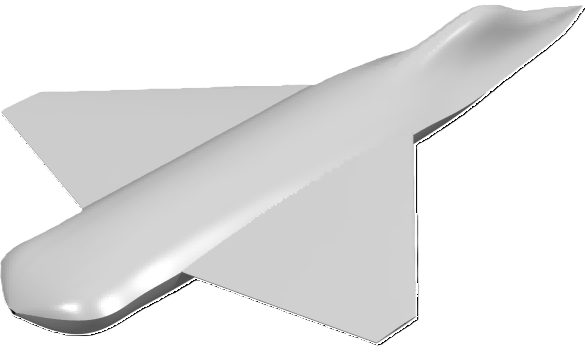
\includegraphics[width=1.5cm,angle=-15]{chapters/images/gfa/baseline-view.png}};
        \draw[tdplot_rotated_coords,dummy] (O) -- (0,0,0.5) node[anchor=south,nuta]{$R$};
        \tdplotsetrotatedthetaplanecoords{0}
        \tdplotdrawarc[tdplot_rotated_coords,circle,nuta]{(0,0,0)}{1}{0}{360}{}{}
        \tdplotdrawarc[tdplot_rotated_coords,elgna,nuta]{(0,0,0)}{\rang}{90-\ephi}{0}{anchor=west,nuta}{$\phi$}
    \end{tikzpicture}
\end{document}